\documentclass[14pt, fleqn, xcolor={dvipsnames, table}]{beamer}
\usepackage[T2A]{fontenc}
\usepackage[utf8]{inputenc}
\usepackage[english,russian]{babel}
\usepackage{amssymb,amsfonts,amsmath,mathtext}
\usepackage{cite,enumerate,float,indentfirst}
\usepackage{cancel}

\usepackage{tikz}                   
\usetikzlibrary{shadows}

% \usepackage{enumitem}
% \setitemize{label=\usebeamerfont*{itemize item}%
%   \usebeamercolor[fg]{itemize item}
%   \usebeamertemplate{itemize item}}

\graphicspath{{images/}}

\usetheme{Madrid}
\usecolortheme{seahorse}
\renewcommand{\CancelColor}{\color{red}}

\setbeamercolor{footline}{fg=Blue!50}
\setbeamertemplate{footline}{
  \leavevmode%
  \hbox{%
  \begin{beamercolorbox}[wd=.333333\paperwidth,ht=2.25ex,dp=1ex,center]{}%
    И. Кураленок, Н. Поваров, Яндекс
  \end{beamercolorbox}%
  \begin{beamercolorbox}[wd=.333333\paperwidth,ht=2.25ex,dp=1ex,center]{}%
    Санкт-Петербург, 2013
  \end{beamercolorbox}%
  \begin{beamercolorbox}[wd=.333333\paperwidth,ht=2.25ex,dp=1ex,right]{}%
  Стр. \insertframenumber{} из \inserttotalframenumber \hspace*{2ex}
  \end{beamercolorbox}}%
  \vskip0pt%
}
\newcommand\indentdisplays[1]{%
     \everydisplay{\addtolength\displayindent{#1}%
     \addtolength\displaywidth{-#1}}}
\newcommand{\itemi}{\item[\checkmark]}

\title{Генеративные вероятностные модели:\\\small{на примере текстов: NB, LSI, PLSI, LDA}}
\author[]{\small{%
И.~Куралёнок,
Н.~Поваров}}
\date{}

\begin{document}

\begin{frame}

\maketitle
\small
\begin{center}
\vspace{-60pt}
\normalsize {\color{red}Я}ндекс \\
\vspace{80pt}
\footnotesize СПб, 2013
\end{center}
\end{frame}

\begin{frame}{Немного о статистической обработке текстов}
Пара фактов:
\begin{itemize}
  \item Нужно исходно для поиска
  \item Область называется Information Retrieval (SIGIR/CIKM/ECIR/РОМИП/RCDL/Диалог)
  \item Читать ``Modern Information Retrieval'', Ricardo Baeza-Yates, Berthier Ribeiro-Neto
\end{itemize}
Из всего этого добра нам сегодня нужно только ``bag of words''.
\end{frame}

\section{Проблема представления документа}
\begin{frame}{Как можно представить текст}
В IR:
\begin{description}
  \item[Документ:] последовательность абзацев
  \item[Абзац:] последовательность предложений
  \item[Предложение:] бог знает что такое, но со словами внутри
\end{description}
К черту подробности! Документ --- банка со словами, которую еще и потрясли.\\ Банка бывает: бинарная, частотная, нормированная, BM25, TFIDF, etc.
\end{frame}

\section{Наивный байес, LSI}

\begin{frame}{Наивный байесов классификатор}
Даже в такой простой модели можно делать например так:
$$\begin{array}{ll}
p(c|d) &= {p(c)\prod_{w_i} p(c|w_i, w_{i-1}, \ldots, w_1) \over \prod_{w_i} p(w_i)} \\
& = \frac{1}{Z} p(c) \prod_{w_i} p(c|w_i)
\end{array}$$
Такая штука называется ``наивный байес'' и долгое время считаласть стандартом де-факто текстового классификатора.
\end{frame}

\begin{frame}{Вспоминая прошлую лекцию (LSI)}
\small
Сложим всю коллекцию документов $X = (d_1,\ldots,d_m)^T$. Каждый документ: $d_i = (w_1, \dots, w_n)$, где $w_i$ --- частота слова в документе. Матрица разряжена, можно попробовать проделать фокус из прошлой лекции:
$$
X = U^T_r \Sigma_r V_r
$$
Тогда вектора в $U_r$ и $V_r$, можно рассматривать как образы слов и документов в общем пространстве гипотез размерности $r$. Будем предсказывать по словам запроса (клиентам) документы (товары), которые соответсвуют предыдущим покупкам (документам, где слово засветилось).
\end{frame}

\section{Смеси распределений и генеративные модели}

\begin{frame}{LSI в терминах вероятностей}
\small
Мы знаем (уже), что SVD разложение работает ``не очень'', может быть можно все переложить в плоскость вероятностного моделелирования по следующей схеме:
\begin{itemize}
  \item сформулируем способ получить документ с помощью некого случайного процесса;
  \item подберем параметры процесса так, чтобы наилучшим способом объяснить появление коллекции;
  \item для нового документа найдем вероятность быть ``сгенерированным'' полученной моделью.
\end{itemize}
Параметров распределения может быть сильно меньше, чем данных в коллекции и в этом смысле мы делаем ``понижение ранга'' модели. Чтобы описывать это безобразие нам помогут графические модели.
\end{frame}

\begin{frame}{Вероятностные модели}
\begin{center}
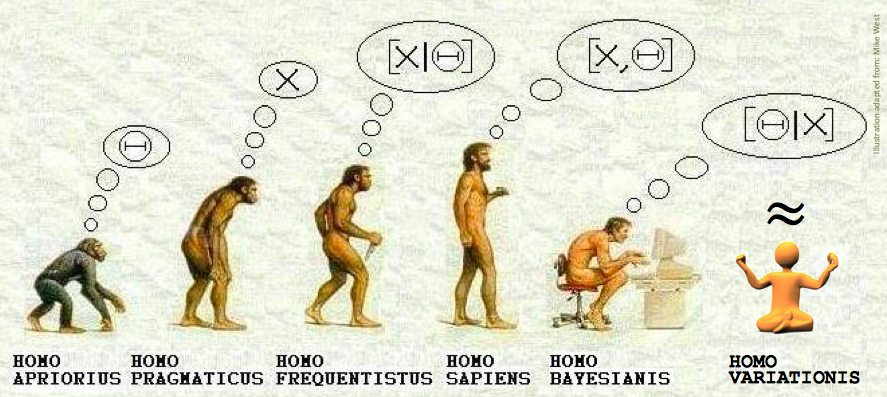
\includegraphics[width=0.9\textwidth]{levels.png}
\end{center}
\footnotesize{картинка из презентации Kay Р. Brodersen}
\end{frame}


\subsection{Униграмная модель}

\begin{frame}{Униграммная модель}
\begin{center}
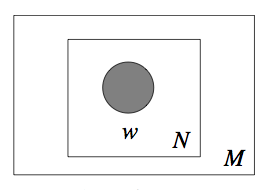
\includegraphics[height=0.3\textheight]{Unigram.png}
\end{center}
$$
p(d) = \prod_{w_i} p(w_i)
$$
\begin{enumerate}
  \item Кинем количество слов $n$ по Пуассону
  \item По полученному количеству будем независимо и с повторениями выбирать слова $p(w_i)$
\end{enumerate}
\end{frame}

\begin{frame}{Униграммный классификатор}
\begin{enumerate}
\footnotesize
  \item поделим коллекцию на классы;
  \item для каждого класса подберем параметры униграммной модели;
  \item по новому документу сравним вероятности быть сгенерированным по соответсвующей классу модели.
\end{enumerate}
$$\begin{array}{ll}
p(d|c) &= \prod_{w_i} p(w_i|c)
\end{array}$$
Чем отличается от Naive Bayes?
\end{frame}

\subsection{Униграмная тематическая модель}

\begin{frame}{Смесь униграмм}
\small
\begin{center}
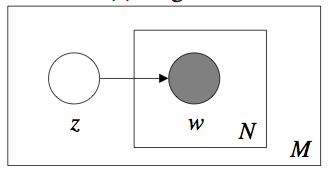
\includegraphics[height=0.3\textheight]{Mixture.png}
\end{center}
$$\begin{array}{ll}
p(d) &= \sum_{z}p(z)\prod_{w_i} p(w_i|z)
\end{array}$$
\begin{enumerate}
  \item Кинем топик $z$ по весам $p(z)$
  \item Кинем количество слов $n$ по Пуассону
  \item По полученному количеству будем независимо и с повторениями выбирать слова с вероятностями $p(w_i|z)$
\end{enumerate}
Документ может относиться только к одной скрытой теме $z$.
\end{frame}

\begin{frame}{Как подбирать смесь униграмм?}
Пускай класс документа является скрытой переменной.
\begin{description}
  \item[Expectation] исходя их текущих представлений о $p(w_i|z)$ найдем к какому классу пренадлежит документ
  \item[Maximization] с учетом того, как распределились документы по классам, максимизируем правдоподобие коллекции
\end{description}
\end{frame}

\subsection{pLSA}
\begin{frame}{Probabilistic latent semantic allocation (pLSA)}
\begin{center}
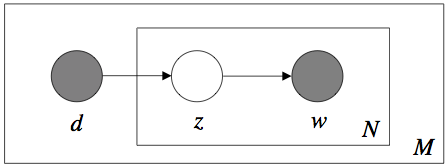
\includegraphics[height=0.3\textheight]{pLSA.png}
\end{center}
\begin{enumerate}
  \item Выберем для документа топик $z$ по весам $p(z|d)$
  \item Кинем количество слов $n$ по Пуассону
  \item По полученному количеству будем независимо и с повторениями выбирать слова с вероятностями $p(w_i|z)$
\end{enumerate}
\end{frame}

\subsection{LDA}
\begin{frame}{Latent Dirichlet Allocation (LDA)}
\begin{center}
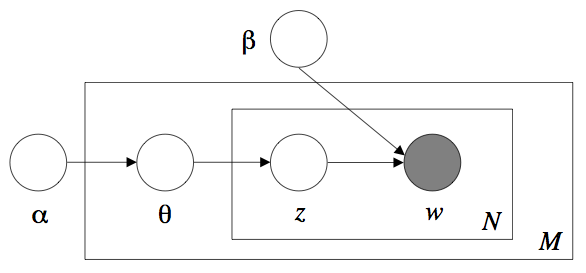
\includegraphics[height=0.3\textheight]{LDA.png}
\end{center}
\begin{enumerate}
  \item Сгенерируем распределения весов топиков $\theta \sim Dir(\alpha)$
  \item Кинем количество слов $n$ по Пуассону
  \item Для каждого слова:
  \begin{enumerate}
    \item Выберем $z_i \sim Multinomial(\theta)$
    \item Получим слово с вероятностью $p(w|z_i,\beta)$
  \end{enumerate}
\end{enumerate}
\end{frame}

\begin{frame}{Вывод LDA I}
\small
Теперь все стало сильно сложнее:
$$
p(d|\alpha, \beta) = \int p(\theta | \alpha)\left(\prod_1^n\sum_{z}p(z_i|\theta)p(w_i|z_i,\beta)\right) d\theta
$$
Или, с учетом известных распределений:
$$
p(d|\alpha, \beta) = \frac{\Gamma\left(\sum_i\alpha_i)}{\prod_i \Gamma(\alpha_i)} \int \left(\prod_{t=1}^k \theta^{\alpha_t-1}_i\right)\left(\prod_{i=1}^n\sum_{t=1}^k\prod_{j=1}^m(\theta_t\beta_{tj})^{w_i^j}\right)d\theta
$$
А для коллекции еще и так:
$$
\arg \max_{\alpha, \beta} \sum_d \log p(d|\alpha, \beta)
$$
\end{frame}

\begin{frame}{Variational bayes}
$$\begin{array}{ll}
\log(p(d)) &= \log(\frac{p(y,\theta)}{p(\theta|y)}) \\
&= \int q(\theta) \log \frac{p(y,\theta)}{p(\theta|y)} d\theta \\
&= \int q(\theta) \log \frac{p(y,\theta)}{p(\theta|y)}\frac{q(\theta)}{q(\theta)} d\theta \\
&= \int q(\theta) \left(\log \frac{q(\theta)}{p(\theta|y)} + \log \frac{p(y,\theta)}{q(\theta)}\right) d\theta \\
&= {\color{red}\left(\int q(\theta) log \frac{q(\theta)}{p(\theta|y)}d\theta\right)} + {\color{blue}\left(\int q(\theta) log \frac{p(y,\theta)}{q(\theta)} d\theta\right)} \\
\end{array}$$
Красная часть называется Kullback–Leibler divergence ($KL(p\|q)=D_{KL}(p\|q)$). Можно искать не точное распределение $p$, а его приближение $q$.
\end{frame}

\begin{frame}{Вывод LDA II}
В нашем случае $q$ выберем так:
$$
q(\theta,z|\gamma,\phi) = q(\theta|\gamma) \prod_{i=1}^n q(z_i | \phi_i)
$$
где $\gamma \sim Dir$, и решим проблему:
$$
(\hat{\gamma},\hat{\phi}) = \arg \min_{(\gamma,\phi)} D_{KL}(q(\theta,z|\gamma,\phi)\|p(\theta, z|d,\alpha,\beta))
$$
\end{frame}

\begin{frame}{Вывод LDA III}
\begin{description}
  \item[Expectation:] для каждого документа найдем параметры $\{\hat{\gamma}, \hat{\phi}\}$
  \item[Maximization:] используя $q(\theta,z|\hat{\gamma}_d, \hat{\phi}_d)$ вместо $p(\theta,z|d,\alpha, \beta)$ максимизируем исходный likelihood
\end{description}
\end{frame}

\begin{frame}{Задание на дом}
\begin{itemize}
  \item Задание будет в svn.
  \item Домашнее задание за пятую неделю ещё проверяется, но пока - "ужас-ужас".
\end{itemize}
\end{frame}
\end{document}
